%!TEX root = ../thesis.tex
% ******************************* Thesis Appendix A ****************************

\ifpdf
    \graphicspath{{Appendix1/Figs/Raster/}{Appendix1/Figs/PDF/}{Appendix1/Figs/}}
\else
    \graphicspath{{Appendix1/Figs/Vector/}{Appendix1/Figs/}}
\fi

\chapter{Appendixed Methods}
\section{Measuring focal length of scan lens}\label{appendix:scanlens}

The focal length of the scan lens was initially unknown but its position for collimation was, and so a reasonable assumption of its focal length was possible.
To compound certainty the focal length was found experimentally.
To accurately measure the focal length of an unknown lens the focal length of a lens of known focal length is needed to collimate the light.
In this experiment the tube lens of focal length \SI{200}{\milli\meter} was used.
By measuring the width of a laser beam prior ($w_{before}$) to and after ($w_{after}$) the collimating lens pair, the magnification is calculated very accurately and the unknown focal length is found by:

\begin{align}
	M=\frac{f_2}{f_1}=\frac{w_{before}}{w_{after}}  \rightarrow \frac{f_2}{M} =f_{1}
\end{align}

To measure a beam width very accurately a straight sharp edge is placed in the beam path and slowly iterated through, the resultant beam power is then measured using a power meter.
To ensure there is no beam cropping on the power meter another lens was used to focus the intensity correctly, the same lens and its position was used in each measurement to keep with consistency.
The beam power was measured and plotted which produces an integrated Gaussian profile (see \eqref{eq:guass_prop}) otherwise known as an error function.
Mathematically this is described by equation \eqref{eq:knife}.

\begin{align}
	I(x,y) &= I_0 e^{\frac{-2x^2}{w_x^2}}e^{\frac{-2y^2}{w_y^2}}\label{eq:guass_prop}\\\nonumber
	P_{TOT} &= I_0 \int_{\infty}^{\infty}e^{\frac{-2x^2}{w_x^2}} dx \int_{\infty}^{\infty}e^{\frac{-2y^2}{w_y^2}} dy\\\nonumber
	P(X) &= P_{TOT} - \int_{\infty}^{X}e^{\frac{-2x^2}{w_x^2}} dx I_0 \int_{\infty}^{\infty}e^{\frac{-2x^2}{w_x^2}} \\\nonumber
	&= \frac{P_{TOT}}{2} - \sqrt{\frac{\pi}{2}} I_0 \omega_y \int_{\infty}^{X}e^{\frac{-2x^2}{w_x^2}}\\
	& = \frac{P_{TOT}}{2} \left[1 - erf\left(\frac{\sqrt{2}X}{\omega_x}\right) \right] \label{eq:knife}
\end{align}

Fitting of this curve was implemented using MatLAB's curve fitting package which utilises the method of least squares fitting, see Figure \ref{eq:emission}.
The fit result produced values of laser beam width as $w_{before} = \SI{3.76\pm0.04}{\milli\meter}$ and $w_{after} = \SI{0.71\pm0.1}{\milli\meter}$.
The value of $w_{after}$ was supplied in Table \ref{table:laser} however, for posterity is was remeasured locally in case the value had changed or was incorrect.
This gives a magnification $M$ of \SI{5.37 \pm 0.1}{} therefore the focal length of the scan lens is \SI{37.3\pm0.1}{\milli\meter}.
This also showed that the fill of the \SI{12}{\milli\meter} back aperture was \SI{3.76\pm0.04}{\milli\meter} hence the NA of the \num{0.3} objective used would be \SI{\approx 0.094}{}.

\begin{figure}
\centering
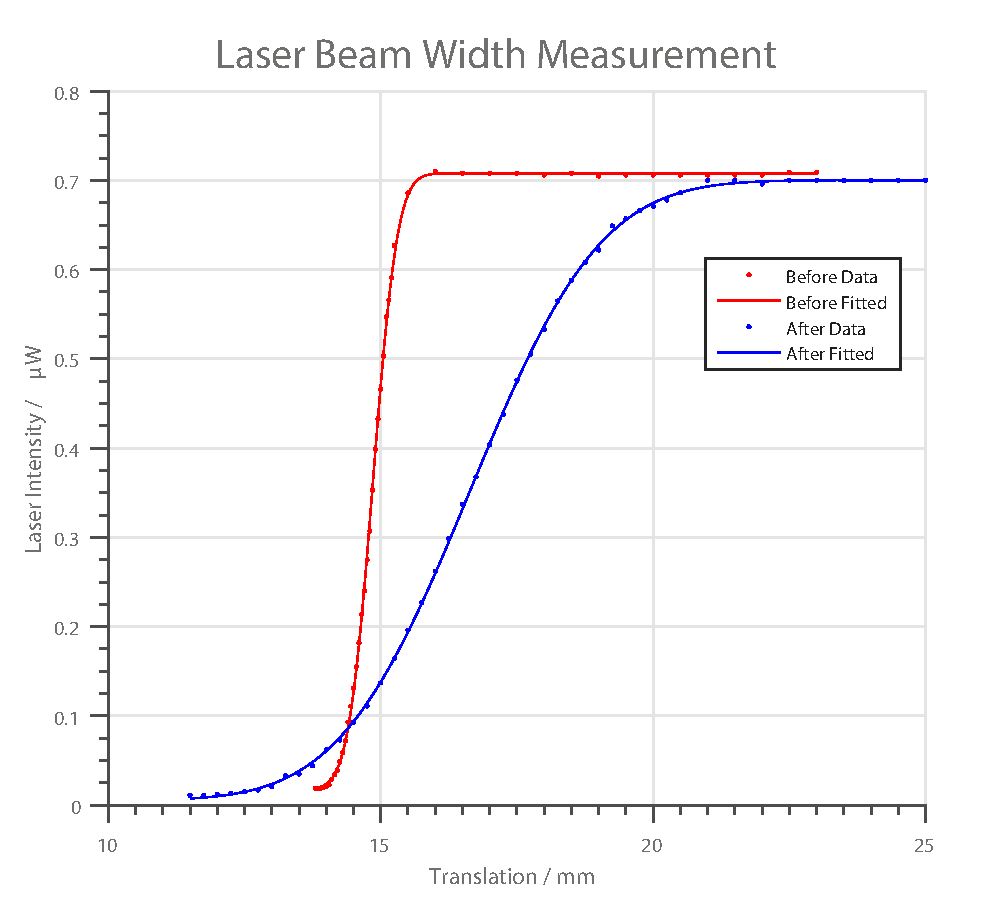
\includegraphics[width=0.7\linewidth]{./laser_width}
\caption[Laser Width Fitting]{Plot showing the fitting of two error functions based on the knife edge translation through a laser beam propagation, producing laser beam widths of $w_{after} = \SI{0.71\pm0.1}{\milli\meter}$ and $w_{before} = \SI{3.76\pm0.04}{\milli\meter}$}
\label{fig:laser_width}
\end{figure}

\section{System alignments protocol}

%Stationary back apeture.

\section{Convolution Theorem}\label{appendix:convolution_theorem}



Convolution is a mathematical operation between two functions, say $g(t)$ and $f(t)$, with the resultant function being an expression of the overlap of $g$ as it is shifted over $f$ \cite{Bracewell1921-}. Mathematically it can be expressed as an integral over a finite range $\tau$:
\begin{equation}
[f(*g](t) = \int_{-\infty}^{\infty} f(\tau) g(t-\tau)d\tau
\end{equation}

If a Fourier transform is then applied to the convolution of two functions:
\begin{align}
\mathcal{F}([f*g](t)) &= \int_{-\infty}^{\infty} \left[{\int_{-\infty}^{\infty} f(\tau)} g(t-\tau)d\tau\right] e^{-i2 \pi kt} dt \\
\text{and then reverse}&\text{ the order:}\nonumber\\
\mathcal{F}([f*g](t)) &= \int_{-\infty}^{\infty}f(\tau) \left[{\int_{-\infty}^{\infty} } g(t-\tau) e^{-i2 \pi kt} dt\right]   d\tau
\\
\text{From the shift theorem}& \text{ seen in equation \eqref{shift_ivariance}:} \nonumber
\\
\left[{\int_{-\infty}^{\infty} } g(t-\tau) e^{-i2 \pi kt} dt\right] &= \mathcal{F}(g(t-\tau)) = \mathcal{F}(g(t)) e^{-i2 \pi k \tau}\\
\implies \mathcal{F}([f*g](t)) &= \mathcal{F}(g(t)) \int_{-\infty}^{\infty}f(\tau) e^{-i2 \pi k \tau}    d\tau
\\&= \mathcal{F}(g(t)) \mathcal{F}(f(\tau)) \label{convolv}
\end{align}

Showing that \textbf{Convolution} in real space is \textbf{Multiplication} is Fourier space.


\section{Fourier transform}

Any continuous function can be decomposed into a linear summation of harmonic weighted sinusoidal functions. A Fourier transform is a mechanism by which the weightings of this series can be derived. Fourier space uses this transform to represent a function or a signal in frequency space (sometimes known as $k$-space or reciprocal space); it can be seen as a coordinate change from $x$ to $k$ denoted mathematically as:  \cite{Bloomfield1946}
\begin{equation}
F(k) \equiv\mathcal{F}  \{f(x)\} \equiv \int_{-\infty}^{\infty}f(x) e^{-i2 \pi kx} dx \label{fourier trans}
\end{equation}

This process is also reversible by:

\begin{equation}
f(x) \equiv\mathcal{F}^{-1}  \{F(k)\} \equiv \frac{1}{2 \pi} \int_{-\infty}^{\infty}F(k) e^{-i2 \pi kx} dk
\end{equation}


Fourier transforms have a valuable property in that a shift in real space becomes a complex phase term in $k$ space. This is shown by substituting $x = x-a$ and $dx = dx$ into \eqref{fourier trans}:
\begin{align}
F(k') &=  \int_{-\infty}^{\infty}f(x) e^{-i2 \pi k(x-a)} dx \nonumber\\
&=  e^{-i2 \pi ka} \underbrace{\int_{-\infty}^{\infty}f(x) e^{-i2 \pi kx}dx}_{F(k)}   \label{shift_ivariance}
\end{align}

Hence the additional real space shift only adds a multiplicative factor to the final Fourier transform. This is known as the Shift theorem.

\section{Huygens}


Diffraction is the spreading of light rays after an interaction with an object. Coincident light waves may interfere when diffracted such that the superposition of their resultant waves is constructive or destructive dependent on their relative phase difference. Light incident on an aperture $A(x,y)$ in the plane $S$ can be assumed to be of a plane wave nature. When passing through the aperture, light can then be modelled as being a series of $dS$ spaced point sources that radiate spherical wavefronts under Huygens' principle:

\begin{quote}
``Every point on a propagating wavefront serves as the source of secondary spherical wavelets, such that the wavefront at some later time is the envelope of these wavelets.'' \cite{Goodman2005}
\end{quote}

%
% \begin{figure}
% \centering
% \includegraphics[width=0.7\linewidth]{./Diagrams/coordsys}
% \caption{Diagram depicting the coordinate system discussed Section \ref{diffraction}.}
% \label{fig:coordsys}
% \end{figure}

The superposition and hence summation of these emitting wavelets when only travelling forward ($+z$ direction) and contained in a cone of small angles from the optical axis can be evaluated in terms of $dE$, the change in the field at some point in front of the aperture. The change in field goes with $\frac{1}{r}$ where $r$ represents the distance to an arbitrary point and for a real wave can be expressed as:

\begin{equation}
dE = \frac{A(x,y)dS}{r} cos(\omega t -kr)
\end{equation}

Using the coordinates $\alpha,\beta$ to represent the two dimensional plane of the projection of the light passing through the aperture $A(x,y)$ then $r$ and $R$ can be written as:
\begin{align}
R^2 &= \alpha ^2 + \beta ^ 2+ z^2  \\
r^2 &= (\alpha - x)^2 + (\beta - y)^2 + z^2
\end{align}
Where $R$ represents the distance from the optical centre of the aperture to the arbitrary point at $\alpha,\beta$, which can be rewritten as:

\begin{equation}
r = R \sqrt{1 - \frac{2 \alpha x + 2 \beta y}{R^2} + \frac{x^2 + y^2}{R^2}}  \label{r = R}
\end{equation}

Which can be approximated using a binomial expansion to:

\begin{equation}
r = R - \frac{(\alpha x + \beta y)}{R}
\end{equation}

Provided the cone of angles is small, then $r \approx R$ and when only considering the case where $R^2 >> x^2 + y^2$ equation \eqref{r = R} tends to:
\begin{equation}
dE = \frac{A(x,y)}{R} e^{i \omega t - kr} e^{ik \left(\frac{\alpha x + \beta y}{R}\right)} dxdy
\end{equation}

Integrating across the entire aperture (wavefronts are entirely rejected elsewhere):


\begin{align}
E(\alpha,\beta) &= \frac{e^{i \omega t - kr}}{R} \int\int_{A}^{} A(x,y) e^{ik \left(\frac{\alpha x + \beta y}{R}\right)} dxdy
\\  \text{After a normalised } &\text{coordinate switch:} \nonumber \\
u &= \frac{k \alpha}{2 \pi R}  \text{ and }   v = \frac{k \beta}{2 \pi R}
\\ E(u,v)&=\frac{e^{i \omega t - kr}}{R} \int\int_{A}^{} A(x,y) e^{i2 \pi k \left(ux + vy\right)} dxdy
\end{align}

This form is well known and defined as a Fourier transform (with a weighting term) and hence the far field diffraction pattern of an aperture is the Fourier transform of that aperture \cite{Goodman2005}.
